\chapter{Bases de Datos Temporales}  \label{cap:t}

\section{Introducción}

% Intro
Estudiaremos ahora el problema de representar \concept{datos temporales} y \concept{relaciones temporales} entre datos,
ambos aspectos muy importantes de los fenómenos del mundo real.
La habilidad de modelar esta dimensión temporal es esencial para aplicaciones informáticas como
econometría, bancos, control de inventario, contabilidad, leyes, registros médicos, sistemas de reservas de vuelos y muchas otras.

% DBs tradicionales: unico estado presente
Podemos introducir la idea de bases de datos temporales como una generalización a la siguiente intuición.
Una base de datos tradicional representa el estado del sistema en un momento específico: el presente.
La existencia de datos que existieron en el pasado o relaciones que fueron verdaderas previamente pero ya no lo son,
quedan relegadas a la lógica de la aplicación del usuario y no poseen soporte del motor de base de datos.

Además, existe otro problema con notables similitudes. A medida que los datos se modifican, las versiones anteriores se pierden.
Los datos desactualizados son borrados de la base de datos.

Surge entonces la problemática de las aplicaciones para las cuales nos sería útil almacenar y razonar sobre estos estados que
si bien no son una representación del estado actual de la realidad modelada, representan igualmente información valiosa.

A lo largo de este capítulo exploraremos estas cuestiones.
En la sección \ref{sec:dominio:tiempo}, introduciremos algunos conceptos lógica temporal.
Luego, en la sección \ref{sec:val:trans} exploraremos en mas detalle los dos tiempos que acabamos de introducir
y que llamaremos tiempo de validez y tiempo de transacción.
Por último, en la sección \ref{sec:sql2011} veremos como estos conceptos fueron introducidos en el estándar SQL 2011.

\section{El dominio del tiempo}\label{sec:dominio:tiempo}

% Intro
Para poder plantear una implementación de una base de datos temporal es necesario comprender primero
cómo se comporta y cómo se observa el tiempo.

% Something something empieza teórico
En el capítulo anterior vimos como la investigación de bases de datos espaciales se vio motivada por
la necesidad práctica de mejorar el manejo de datos de los sistemas GIS.
Las bases de datos temporales por su parte, fueron fuertemente impactadas por
la investigación previa en lógica temporal desde de los años 70\textsuperscript{\cite{temporal:status:directions}}
y que presentaremos a continuación.

\subsection{La estructura del tiempo}

Los trabajos fundacionales de la lógica temporal han dividido el estudio del tiempo en dos modelos estructurales principales:
\concept{lineal} y \concept{ramificado}\textsuperscript{\cite{temporal:snodgrass}}.
Comenzaremos entonces por estudiar estos modelos y luego mencionaremos brevemente otras posibilidades.

\subsubsection{Modelo Lineal}

Es el modelo más simple, donde el tiempo avanza del pasado al futuro de forma ordenada formando así una secuencia
tal y como se ve en la figura \ref{fig:linear-time-model}.

\begin{figure}
    \centering
    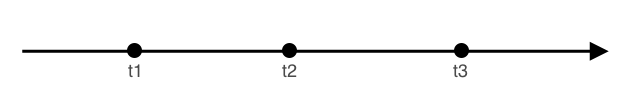
\includegraphics[scale=0.5]{fig-linear-time.png}
    \caption{Ejemplo de modelo lineal del tiempo}
    \label{fig:linear-time-model}
\end{figure}

Generalmente esta estructura es útil para mantener información histórica centrada en eventos del pasado.
Por ejemplo: registros de transacciones de un banco, sistemas de control de inventario, etc.

\subsubsection{Modelo ramificado}

A diferencia del modelo anterior, el tiempo se presenta en dos formas:
se extiende de forma lineal desde el pasado hacia el presente formando una secuencia
y se ramifica del presente al futuro creando un árbol con raíz en el \textit{ahora} cuyas ramas se extienden hacia el futuro.
Podemos visualizar este modelo en la figura \ref{fig:branched-time-model}.

\begin{figure}
    \centering
    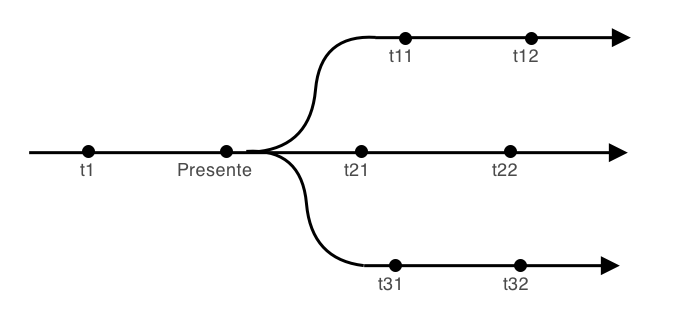
\includegraphics[scale=0.5]{fig-branched-time.png}
    \caption{Ejemplo de modelo ramificado del tiempo}
    \label{fig:branched-time-model}
\end{figure}

A esta forma de organizar el tiempo también se la conoce con el nombre de “modelo de los posibles futuros”.
Debido a sus características es útil para representar y trabajar con información predicativa.

\subsubsection{Elección entre estructuras temporales}

Los modelos más generales del tiempo en la lógica temporal representan el tiempo como un conjunto arbitrario
que cumple con la restricción de ser un \textit{orden parcial}.
Otros axiomas introducen otros modelos más refinados del tiempo.
Por ejemplo: el tiempo lineal puede ser simplificado agregando un axioma que imponga un \textit{orden total} en este conjunto.
Un modelo recurrente, por otra parte, puede trabajarse con un \textit{modelo cíclico} del tiempo.

A lo largo de este capítulo se utilizará un modelo lineal del tiempo ya que es el más sencillo
y brinda todas las características necesarias en las bases de datos temporales.

\subsection{La densidad del tiempo}

%TODO citas aca cuando tenga las citas del pelotudo de Snodgrass
Siguiendo con el modelo lineal, la densidad del tiempo puede variar en la línea.
Esta se puede clasificar en dos grupos: \concept{discretos} y \concept{densos}.

\subsubsection{Modelos Discretos}

Estas representaciones son isomorfas a los números naturales, lo cual implica que cada punto en el tiempo tiene un único sucesor.
Cada número natural corresponde a una unidad no descomponible de tiempo de duración arbitraria.
Estas reciben el nombre de \concept{chronons}.

\subsubsection{Modelos Densos}

Por su parte, los modelos densos presentan dos variaciones: pueden ser isomorfos tanto a los números racionales como a los reales.
Como consecuencia, dados dos momentos cualquiera en el tiempo, existe otro momento entre ellos.

Los modelos isomorfos a los reales también son conocidos como continuos.

\subsubsection{\textit{Chronons} y la elección del modelo de densidad}

Un \concept{chronon} es la duración de tiempo más pequeña que puede ser representada.
Cabe destacar que no se trata de un punto sino un segmento en la línea del tiempo.
A pesar de que el tiempo en sí mismo suele ser percibido como algo continuo,
la mayoría de las propuestas para agregar una dimensión temporal a los modelos de datos relacionales están basados en un modelo discreto del tiempo.
Existen varias razones para esta elección entre las que se destacan cuatro:

\begin{itemize}
    \item Las medidas del tiempo son inherentemente imprecisas.
    Los instrumentos de medición temporal invariablemente reportan la ocurrencia de eventos en términos de chronons, no en “puntos” de tiempo.
    Por lo tanto, incluso los eventos así llamados “instantáneos” pueden ser medidos como si hubieran ocurrido durante un chronon, en el mejor de los casos.
    \item La mayor parte de las referencias temporales del lenguaje natural son compatibles con el modelo discreto del tiempo.
    Por ejemplo, cuando se dice que un evento ocurrió a las 4:30 PM,
    en realidad no se hace referencia a que el evento ocurrió en el “punto” del tiempo asociado a las 4:30 PM,
    sino a algún momento cercano a las 4:30 PM aunque exista una variación de uno o dos minutos.
    \item Los conceptos de chronon y de intervalo permiten modelar naturalmente eventos que no son instantáneos sino que tienen duración.
    \item Cualquier implementación de un modelo de datos con dimensión temporal tendrá la necesidad de codificar el tiempo de forma discreta,
    Es decir que, es inevitable discretizar el tiempo en algún punto.
    Este problema es análogo al que analizamos en el Álgebra de Rose en el capítulo anterior.
\end{itemize}

\section{\textit{Tiempo de Validez} y \textit{Tiempo de Transacción}} \label{sec:val:trans}
%TODO: algun tipo de cita en todo esto. dios mio.

Ahora que hemos introducido los conceptos de la lógica temporal,
pasaremos a la cuestión de integrar estos conceptos a un modelo de bases de datos relacionales.
Como veremos, es útil definir dos categorías fundamentales de datos temporales:
\textbf{tiempo de validez} y \textbf{tiempo de transacción}.

Volviendo sobre la intuición que planteamos en la introducción de este capitulo, llamaremos \concept{bases de datos snapshot} a cualquier base de datos
que no soporta capacidades temporales (independientemente de si tiene datos temporales en un sentido definido por el usuario).
Como se aprecia en la figura \ref{fig:state-machine}, podemos modelar estas bases de datos como maquinas de estado finitas, en la que cada
estado contiene solo los datos del presente y un cambio destruye los datos anteriores.

\begin{figure}
    \centering
    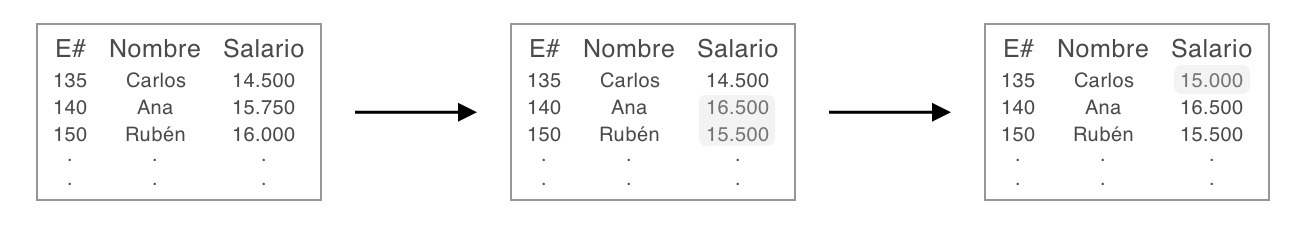
\includegraphics[scale=0.32]{fig-state-machine.jpg}
    \caption{Base de Datos Snapshot como una maquina de estos finita.}
    \label{fig:state-machine}
\end{figure}

Si nos interesa modelar los aspectos temporales propios del dominio del problema,
podemos ampliar este modelo introduciendo el concepto de tiempo de validez,
es decir el tiempo cuando el dato es verdadero en la realidad modelada.
Un dato puede tener asociados múltiples instantes e intervalos de tiempo de validez que representen diferentes atributos temporales del mismo.
A este tiempo también se lo suele conocer como tiempo del mundo real o tiempo lógico.

Por otro lado, si nos interesa mantener un registro histórico de los estados que recorrió la base de datos,
introduciremos el tiempo de transacción, es decir el tiempo en el cual el hecho fue modelado por el usuario.
Llamaremos \concept{consultas de viaje en el tiempo} a aquellas que especifiquen un tiempo de transacción distinto al presente.

Es importante notar que estos dos tiempos no solo cumplen roles distintos y son independientes el uno del uno del otro,
sino que ademas se comportaran distinto.
Generalmente, el tiempo de validez será ingresado por el usuario mientras que
el tiempo de transacción es administrado por el motor de bases de datos.
Como consecuencia de esto, un usuario no puede modificar los estados del pasado.
Llamaremos además \concept{base de datos bitemporal} a una base de datos que soporta ambos tiempos
y \concept{base de datos unitemporal} a aquellas que solo soportan uno de ellos.

\begin{figure}
    \centering
    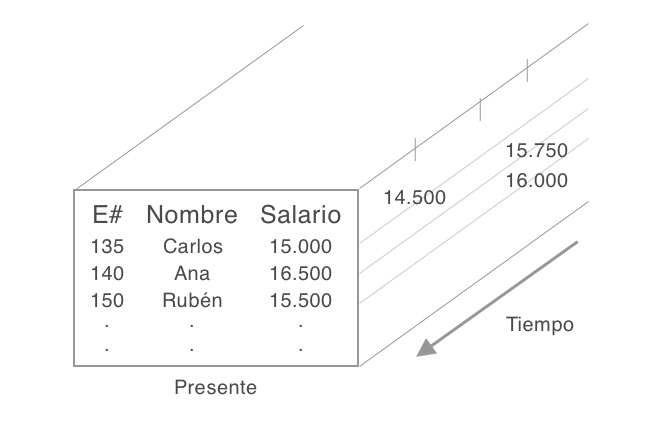
\includegraphics[scale=0.5]{temporal_dimension.jpg}
    \caption{Base de datos con tiempo de transacción.}
    \label{fig:transaction-time}
\end{figure}

\section{Funcionalidades Temporales en SQL 2011}\label{sec:sql2011}

La versión 2011 de SQL\textsuperscript{\cite{sql2011}}, publicada en diciembre de 2011 extiende el estándar con funcionalidades temporales.
Esta extensión se basa en el agregado de \concept{períodos temporales} a las tablas.
La misma define dos variantes de períodos:
de \concept{aplicación de usuario} (para tiempos de validez) y de \concept{versionado del sistema} (para tiempos de transacción).
Los períodos se definen con dos columnas temporales (tipos \textit{Date} o \textit{Timestamp}) de la tabla.
Se prefirió esta forma en lugar de un tipo nuevo ya que es la que permite migrar más
fácilmente sistemas previos al estándar.
Además, como es común en el álgebra temporal, los periodos son \concept{cerrado-abierto},
es decir que contienen el momento de su inicio pero no de su finalización.

\subsection{Períodos de Aplicación de Usuario} \label{subsec:pau}

Veamos ahora un ejemplo de una tabla que define un periodo de aplicación de usuario:

\begin{verbatim}
    CREATE TABLE Estudiantes (
        Legajo INTEGEER,
        EStart DATE,
        EEnd DATE,
        ECarrera INTEGER,
        PERIOD FOR EPeriod (EStart, EEnd)
    );
\end{verbatim}

Como vemos, las columnas \texttt{EStart} y \texttt{EEnd} son respectivamente el comienzo y fin del período \texttt{EPeriod}.
Como mencionamos en la sección anterior, al tratarse de un tiempo de validez debe poder ser establecido por el usuario.
Efectivamente, podemos especificar los valores de este período y de hecho,
la sintaxis para hacerlo no cambia en nada respecto a un \texttt{INSERT} tradicional.

\begin{verbatim}
    INSERT INTO Estudiantes
    VALUES (1234, DATE '2013-03-01', DATE '2018-12-20', 1);
\end{verbatim}

Consideremos ahora la tabla con esta fila y veamos una query un poco mas interesante.

\begin{verbatim}
    UPDATE Estudiantes
        FOR PORTION OF EPeriod
            FROM DATE  DATE '2015-04-01'
            TO DATE '2015-05-01'
    SET Carrera = 2
    WHERE Legajo = 1234;
\end{verbatim}

Lo primero que notamos en este \texttt{UPDATE} es que introducimos una sintaxis nueva que nos permite establecer
en que tiempo de validez debe ser actualizado el valor.
En este caso, el período especificado está contenido en el período de la fila presente en la tabla.

Pero entonces, ¿Cuál debería ser el nuevo período de validez de la fila actualizada?
La respuesta es que en realidad, un \texttt{UPDATE} temporal se comporta un poco distinto uno tradicional.
O, mas precisamente, es una generalización de este.
Si consideramos que un \texttt{UPDATE} clásico inserta una fila en la tabla por cada una que remueve,
un \texttt{UPDATE} temporal puede crear varias filas (hasta tres) por cada una que borra.
En este caso, por ejemplo, el resultado serán tres filas, como vemos en la tabla \ref{tab:update}.
De todas formas, si la tabla tuviera definidos triggers para las actualizaciones,
la fila con \texttt{carrera = 2} se considera como la actualizada.

\begin{table}[]
    \center \begin{tabular}{l|l|l|l}
    Legajo & EStart     & EEnd       & ECarrera \\ \hline
    1234   & 2013-03-01 & 2015-04-01 & 1        \\
    1234   & 2015-04-01 & 2015-05-01 & 2        \\
    1234   & 2015-05-01 & 2018-12-20 & 1
    \end{tabular}
    \caption{la tabla \texttt{Estudiantes} luego del \texttt{UPDATE}.}
    \label{tab:update}
\end{table}

Similarmente, un \texttt{DELETE} puede borrar un dato en un subperíodo de validez.
%TODO quizas poner un ejemplo. Vemos si necesitamos ocupar mas espacio.

\subsection{Claves Primarias}

Esta nueva semántica de actualizaciones que y borrados nos introduce por otro lado un problema.
En el ejemplo anterior, si la clave primaria de la tabla era el legajo, se produce una duplicación.
Es evidente que tenemos que incluir el período en la PK.

Comúnmente querremos además evitar una forma particular de duplicación en los datos temporales:
filas iguales en la parte no temporal de la clave primaria y con una superposición de periodos.
Para evitar este caso claramente no alcanza con prohibir la igualdad en todas las columnas como en un dato no temporal.
Por este motivo, se introduce la directiva \texttt{WITHOUT OVERLAPS}.
Podemos volver a definir entonces nuestra tabla \texttt{Estudiantes} de la siguiente manera:

\begin{verbatim}
    CREATE TABLE Estudiantes (
        Legajo INTEGEER,
        EStart DATE,
        EEnd DATE,
        ECarrera INTEGER,
        PERIOD FOR EPeriod (EStart, EEnd),
        PRIMARY KEY (
            Legajo,
            EPeriod WITHOUT OVERLAPS
        )
    );
\end{verbatim}


%TODO: outro de tiempo de validez?

\subsection{Períodos de Versionado del Sistema} \label{subsec:pvs}

Como mencionamos previamente, el otro tipo de períodos es de versionado de sistema.
Las tablas declaradas con versionado de sistema tienen campos temporales de nombre fijo (\texttt{sys\_start} y \texttt{sys\_end}),
que el usuario no puede modificar, sino que sus valores son definidos por el sistema al momento de realizar otras operaciones.
El uso de esta funcionalidad es opcional y se declara con la sintaxis WITH SYSTEM VERSIONING.

\begin{verbatim}
    CREATE TABLE Estudiantes (
        Legajo INTEGEER,
        EStart DATE,
        EEnd DATE,
        ECarrera INTEGER,
        PERIOD FOR EPeriod (EStart, EEnd),
        PRIMARY KEY (
            Legajo,
            EPeriod WITHOUT OVERLAPS
        )
    )
    WITH SYSTEM VERSIONING;
\end{verbatim}

Como mencionamos en la sección anterior,
a las consultas por datos en un tiempo del sistema diferente al presente se las conoce como \concept{consultas de viaje en el tiempo}.
Los siguientes son algunos ejemplos de este tipo de consultas.

\begin{verbatim}
    SELECT Legajo, Carrera, sys_start, sys\_end
    FROM Estudiante
    FOR SYSTEM TIME AS OF TIMESTAMP ’2017-05-01 00:00:00’;
\end{verbatim}

\begin{verbatim}
    SELECT Legajo, Carrera, sys_start, sys_end
    FROM Estudiante
    FOR SYSTEM TIME
        FROM TIMESTAMP ’2017-05-01 00:00:00’
        TO TIMESTAMP ’2017-06-01 00:00:00’;
\end{verbatim}


\begin{verbatim}
    SELECT Legajo, Carrera, sys_start, sys_end
    FROM Estudiante
    FOR SYSTEM TIME BETWEEN
        TIMESTAMP ’2017-05-01 00:00:00’
        AND TIMESTAMP ’2017-06-01 00:00:00’;
\end{verbatim}

Vale la pena mencionar brevemente algunos detalles de esta sintaxis.
Por un lado, tenemos dos formas de especificar períodos ya que \texttt{FROM ... TO ...} es Cerrado-Abierto
mientras que \texttt{BETWEEN ... AND ...} es Cerrado-Cerrado.
Por otro, se definen algunas constantes:
una query sin especificar tiempo es equivalente a \texttt{FOR SYSTEM TIME AS OF CURRENT TIMESTAMP}.

Cuando está activada esta funcionalidad, cualquier query \texttt{UPDATE} o DELETE automáticamente preserva el estado anterior en filas nuevas.
Podemos pensar que las filas son de dos tipos,
de \concept{sistema actual} cuando el presente se encuentra dentro de su período de versionado de sistema
e \concept{históricas} en otro caso.
Obviamente, no pueden realizarse queries \texttt{UPDATE} o \texttt{DELETE} sobre filas históricas.

Las restricciones de integridad, por otro lado, son mas sencillas que en el caso de los períodos de aplicación de usuario:
cualquier restriccion que es chequeada y se cumple en el sistema actual, heredará la propiedad cuando pase a ser una versión histórica.

El estándar SQL 2011 soporta además bases de datos bitemporales en el sentido definido en al sección \ref{sec:val:trans},
permitiendo combinar libremente estas funcionalidades con las de tiempo de aplicación de usuario vistas anteriormente.